\documentclass[notitlepage]{report}%{article}

%-- My Definitions
\usepackage{mydefs}

%-- Math stuff
\usepackage{mathtools, amsfonts, amsthm, amssymb}

%-- Phsysics and Chemsitry stuff
\usepackage[version=4]{mhchem}
\usepackage{braket}
\usepackage{siunitx}
\sisetup{input-digits = 0123456789\pi}
\sisetup{separate-uncertainty=true}
%to compile Feynman diagrams: uncomment these
%can take a lot of compile time, set the compiler to LuaLaTex
%\usepackage[compat=1.1.0]{tikz-feynman}
%\usepackage{tikz}
\usepackage{todonotes}
%-- Computer science stuff
\usepackage{algorithm, algpseudocode, minted}

%-- Plotting
\usepackage{graphicx}

%-- Tables and enumerations
\usepackage{enumerate}
\usepackage{booktabs, multirow}
\usepackage{caption, subcaption}

%-- Bibliography
\usepackage{csquotes}
\usepackage{biblatex}
\addbibresource{bibliography.bib}


%-- Numbering
\numberwithin{equation}{section}
\numberwithin{algorithm}{section}
\counterwithin{figure}{section}
\counterwithin{table}{section}


%-- General Formatting
\usepackage[top=20mm,bottom=20mm,left=25mm,right=25mm]{geometry}
\usepackage[english]{babel}
\usepackage[colorlinks=true, allcolors=blue]{hyperref}
\usepackage{fancyhdr}
\usepackage{parskip}
%\setlength{\parindent}{0pt}
%\setlength{\parskip}{0.5\baselineskip}

%-----> Document begins here <-----
\begin{document}

% -- Title page

\title{Specialist Course: Lattice Field Theory \\ Final Project: Comparison of Algorithms}
\author{Fiona Pärli}
\date{\today}

\maketitle
% -- Table of contents
\setcounter{tocdepth}{2}
\tableofcontents

% -- The main body
\chapter{Introduction}
This final project of the Specialist Course "Lattice Field Theory" (by Prof. Dr. Fernando Romero-López and Victor Granados) aims to do a comparison of the Metropolis and the HMC algorithms applied to scalar $\phi^4$ theory using Markov Chain Monte Carlo methods. The main objective is to compare the performance, efficiency, and physical behavior of the Metropolis and Hybrid Monte Carlo (HMC) algorithms.\\\\
The project combines algoritmic and computational aspects. The Metropolis and HMC algorithms were implemented in Python and Rust. For HMC, two integrators (leapfrog and omelyan2) were used and their effect on energy conservation was studied. \\\\
The simulations were carried out for the two-dimensional $\phi^4$ theory in both the symmetric and broken phases. A range of lattice sizes were considered in order to study errors, autocorrelations and observables as functions of $L$. The topological charge was investigated using periodic and anti-periodic boundary conditions in order to probe non-trivial topological effects such as kink–antikink configurations.\\\\
The main conclusion of this final project is that HMC with omelyan2 integrator in Rust provides the most favorable combination of accuracy, efficiency, and low autocorrelation.
\chapter{Scalar \texorpdfstring{$\phi^4$}{phi4} Theory}
Scalar $\phi^4$ theory is the simplest quantum field theory in which we can see spontaneous symmetry breaking of the discrete $\mathbb{Z}_2$ reflection symmetry, $\phi(x) \rightarrow -\phi(x)$. \\\\
The difference between explicit and spontaneous breaking of a symmetry is that with spontaneous symmetry breaking, the Lagrangian is invariant under the symmetry, but the gorund state is not. As a consequence, in spontaneous symmetry breaking, a phase transition occurs. In explicit symmetry breaking, the symmetry was already violated at the level of the Lagrangian. \\\\
For discrete symmetries such as the $\mathbb{Z}_2$ symmetry of $\phi^4$ theory, spontaneous symmetry breaking looks very similar to explicit symmetry breaking. Breaking of a continous global symmetry (for example a global $U(1)$ phase symmetry) would lead to massless particles (Goldstone theorem) and for gauged symmetries, this could explain the Higgs mechanism. However, this is beyond the scope of this project. \cite{SchwartzQFT}\\\\
Strictly speaking, spontaneous symmetry breaking occurs only in the infinite-volume limit. On a finite lattice, tunneling between degenerate vacua restores the symmetry, although for sufficiently large volumes the system behaves effectively as if the symmetry were broken. Furthermore, due to lattice renormalization effects, the critical value of the bare mass differs from its continuum value and must be determined numerically. Near this critical point the correlation length diverges, leading to critical slowing down in Monte Carlo simulations. \cite{SchwartzQFT,GattingerLang}\\\\
This section is provided for completeness and is heavily based on the tutorial of the LFT course and the following book: \cite{SchwartzQFT}.
\section{The \texorpdfstring{$\phi^4$}{phi4} Theory Action}
We work in two-dimensional Euclidian space. Then, the $\phi^4$- theory action is described by the following Lagrangian:
\begin{equation}
    S[\phi] = \int d^2x \left[ \frac{1}{2}(\partial_\mu \phi) (\partial^\mu \phi) + \frac{1}{2} m^2 \phi^2 + \frac{1}{4!}\lambda \phi^4 \right], 
\end{equation} 
where $m^2$ and $\lambda$ are the mass and self-interaction parameters of the theory. We could regard these parameters as being temperature dependent, then this model could describe a system such as a ferromagnet near its critical temperature.\\
Throughout this project, we mostly assume periodic boundary conditions in all dimensions, hence by integrating by parts, we obtain
\begin{equation}
    S[\phi] = \int \mathrm{d}^{2}x \;  \left[ -\frac{1}{2} \phi \left( \partial_{\mu} \partial^{\mu} \phi \right) + \frac{1}{2} m^{2} \phi^{2} + \frac{1}{4!} \lambda \phi^{4} \right].
\end{equation}
The total derivative term vanished because of the periodic boundary conditions. This rewriting shows explicitly that the kinetic energy term becomes a nearest neighbour coupling when discretizing the action. \\\\
In Section \ref{sec:topology}, also anti-periodic boundary conditions will be considered. While periodic boundary conditions preserve tranlational invariance, aperiodic boundary conditions enforece a sign change of the field around the boundary, which introduces a non-trivial topology. This distinction plays an important role in the study of topological properties and allows for the definition of a relative topological charge by comparing configurations generated with different boundary conditions.
\section{Different Masses \texorpdfstring{$m^2$}{m2}}
The action has the following scalar potential: 
\begin{equation}
    V(\phi) = \frac{1}{2}m^2\phi^2 + \frac{1}{4!}\lambda \phi^4. 
\end{equation}
The parameter $\lambda$ has the same dimension as a squared mass.
We assume that $\lambda > 0$ is positive, such that the potential is bounded from below. This is required to define a proper distribution, as it ensures that the Boltzmann weight $e^{-S[\phi]}$ is normalizable. \\\\
This potential can model a system near a phase transition, such as a ferromagnet near the critical temperature $T_c$. The mass parameter $m^2$ plays a role analogous to the inverse correlation length, its sign determines the phase of the system. 
We can imagine the mass to be temperature dependent: 
\begin{equation}
    m^2(T) = c(T - T_c), 
\end{equation}
where $c$ is some positive constant \cite{SchwartzQFT}. \\
We distinguish for the following two cases for the mass parameter: 
\begin{itemize}
    \item If $m^2 \geq 0$ ($T \geq T_c$), the potential has a minimum at $\phi = 0$, which corresponds to a minimum of the action. There is a single vacuum state for which $\braket{\phi} = 0$. The $\mathbb{Z}_2$ symmetry of the theory is preserved. 
    \item If $m^2 < 0$ ($ T < T_c$), $\phi = 0$ is a local maximum and there are two degenerate minima at $\phi = \pm \sqrt{\frac{-6m^2}{\lambda}}$. There are now two vacuum states and $\braket{\phi} = \pm \sqrt{-\frac{6m^2}{\lambda}}$. This is the case of spontaneous symmetry breaking. 
\end{itemize}
Since the vacuum expectation value $\langle \phi \rangle = 0$ is invariant under $\phi \to -\phi$, but the two vacua $\langle \phi \rangle = \pm \sqrt{-6 m^{2} / \lambda}$ are not, this is a case of spontaneous symmetry breaking. That means there occurs a phase transition at some critical mass value $m_c^2 < 0$. At this critical point, the correlation length diverges. This is the point where Monte-Carlo simulations become critical-slowing-down limited. 
\\\\
In this picture, spontaneous symmetry breaking is associated with a continuous phase transition where the effective mass crosses zero. The order parameter $\braket{\phi}$ changes from zero in the symmetric phase to a nonzero value in the broken phase, analogous to the magnetization of a ferromagnet emerging below the Curie temperature.
\\\\
In Euclidian lattice simulations, the temperature does not appear explictly (where for example in the Ising model, it does). Changing $\lambda$ and $m^2$ plays the role of changing extrenal thermodynamical variables. This also shows that the scalar $\phi^4$ theory with its spontaneous $\mathbb{Z}_2$ symmetry breaking mirrors the magnetization transition of the Ising model. For more details about the Ising model, see \cite{WieseThermodynamics}. 
\section{Discretization of Scalar \texorpdfstring{$\phi^4$}{phi4} Theory}
This section is based on the tutorial of the LFT course. \\
We discretize this theory on a two-dimensional spacetime lattice of $L^2$ lattice sites with lattice spacing $a$ and denote the spacetime points as 
\begin{equation}
    \vec{x} = a \vec{n} = a(n_1, n_2), \quad 0 \leq n_1, n_2 < L. 
\end{equation}
We approximate the integral as a sum over all lattice sites: 
\begin{equation}
    \int \mathrm{d}^{2} x \rightarrow a^{2} \sum_{\vec{n}},
\end{equation}
For the discretization of the second derivative, we use the five-point stencil discretization (more on that, see \cite{FivePointStencilWiki}): 
\begin{equation}
    \begin{aligned}
        \partial_{\mu}\partial^{\mu} \phi(\vec{x}) & = \left( \frac{\partial^{2}}{\partial x_{1}^{2}} + \frac{\partial^{2}}{\partial x_{2}^{2}} \right) \phi(\vec{x}) \\
         & \to \frac{\phi(n_{1} + 1, n_{2}) + \phi(n_{1} - 1, n_{2}) + \phi(n_{1}, n_{2} + 1) + \phi(n_{1}, n_{2} - 1) - 4 \phi(\vec{n})}{a^{2}} + \mathcal{O}(a^{2}) \\
         & = \sum_{\mu \in \{1, 2 \} } \frac{1}{a^{2}} \left[ \phi(\vec{n} + \hat{\mu}) + \phi(\vec{n} - \hat{\mu}) - 2 \phi(\vec{n}) \right] + \mathcal{O}(a^{2}).
    \end{aligned}
\end{equation}
All together, the discretized action reads
\begin{equation}
    S[\phi] = a^{2} \sum_{\vec{n}} \left( -\frac{1}{2 a^{2}} \phi(\vec{n}) \sum_{\mu} \left[ \phi(\vec{n} + \hat{\mu}) + \phi(\vec{n} - \hat{\mu}) - 2 \phi(\vec{n}) \right] + \frac{1}{2} m^{2} \phi^{2}(\vec{n}) + \frac{1}{4!} \lambda \phi^{4}(\vec{n}) \right)
\end{equation}
or, after some algebra,
\begin{equation}
    \boxed{S[\phi] = \sum_{\vec{n}} \left( \left[ 2 + \frac{1}{2} m^{2}\right] \phi^{2}(\vec{n}) + \frac{1}{4!} \lambda \phi^{4}(\vec{n}) -\sum_{\mu} \left[ \phi(\vec{n} + \hat{\mu}) \phi(\vec{n})\right] \right)} \label{eq: discrete_action}
\end{equation}
where we have redefined $(am)^{2} \to m^{2}$ and $(a^{2} \lambda) \to \lambda$. The discretized action has a changed mass, $m_{\text{eff}}^2 = 2 + \frac{1}{2}m^2$. This effective mass term includes contributions from the lattice Laplacian. As a consequence, the critical value of the bare mass differs from its continuum counterpart and must be determined numerically. This shift plays an important role in lattice simulations and is closely related to mass renormalization effects \cite{GattingerLang}. 
\chapter{Algorithms}
\section{General Introduction to Monte Carlo Methods}
Our goal is to evaluate the expectation value of an observable $O[U]$ in the quantized Euclidian gauge field theory on a lattice. This is written as a path integral
\begin{equation}
    \braket{O} = \frac{1}{Z} \int \mathcal{D}[U] \; \exp \left( -S[U] \right) O[U], \label{eq: path_integral}
\end{equation}
where the partition function is defined as
\begin{equation}
    Z = \int \mathcal{D}[U] \exp \left( -S[U] \right). \label{eq: partition_function}
\end{equation}
Here, $S[U]$ denotes the Euclidian action and $\mathcal{D}[U]$ represents the functional integration over all field configurations. In the general case, these integrals cannot be solved analytically and depending on the application, these can be high-dimensional \cite{GattingerLang}. \\\\
Using probability theory, we can approximate the integral of a function $f(x)$ by averaging the functional values $f(x_n)$ at values $x_n$, which are randomly chosen according to a uniform distribution 
\begin{equation}
    \rho_u(x_n) = \frac{1}{b-a}. 
\end{equation}
The integral is approximated as: 
\begin{equation}
    \frac{1}{b-a}\int_a^b dx \; f(x) = \lim_{N \rightarrow \infty} \frac{1}{N}\sum_{n=1}^N f(x_n). 
\end{equation}
The exact mean is replaced by the sample mean, the calculation is restricted to a subsample and a finite number $N$. By the Strong Law of Large Numbers, the Monte Carlo estimator
\[
\frac{1}{N} \sum_{n=1}^{N} f(x_n)
\]
converges almost surely to the exact expectation value as $N \to \infty$, and the Central Limit Theorem implies an error scaling of $\mathcal{O}\!\left( \frac{1}{\sqrt{N}} \right)$. This means to increase the accuracy by a factor of two, one has to use four times as many samples \cite{GattingerLang}. 
\subsection{Example of a Simple Monte Carlo Integral}
To illustrate the basic idea of Monte Carlo integration, we consider a simple one-dimensional example. Suppose we want to estimate the integral
\begin{equation}
\int_0^1 \exp(-x^2) \, dx.
\end{equation}
We restrict the upper limit to $1$ to match the support of a uniform random variable. Let $X$ be a random variable uniformly distributed on the interval $(0,1)$. Its probability density function (pdf) is given by
\begin{equation}
f(x) = 
\begin{cases}
1 & \text{if } x \in (0,1), \\
0 & \text{otherwise}.
\end{cases}
\end{equation}
Then the integral can be written as an expectation, 
\begin{equation}
\int_0^1 \exp(-x^2) \, dx = \mathbb{E}[\exp(-X^2)].
\end{equation}
A Monte Carlo estimator using $N$ independent samples $X_1, X_2, \dots, X_N$ from the uniform distribution is
\begin{equation}
I_N = \frac{1}{N} \sum_{i=1}^N \exp(-X_i^2).
\end{equation}
By the law of large numbers, this estimator converges to the true value as $N \to \infty$, 
\[
I_N \xrightarrow[]{N \to \infty} \int_0^1 \exp(-x^2) \, dx.
\]
Moreover, by the central limit theorem, the statistical error scales as $\mathcal{O}\left( \frac{1}{\sqrt{N}}\right)$, which is independent of the dimensionality of the integral. The not scaling with dimension is an important reason for the use of Monte Carlo methods in lattice field theory. This simple example illustrates how Monte Carlo methods approximate integrals by replacing them with sample averages \cite{Monte_carlo}.
\subsection{Importance Sampling}
In our path integral in Equation \ref{eq: path_integral}, we need to account for the Boltzmann factor $\exp(-S)$. This is a weighting factor, depending on the action $S$, of the different field configurations. 
The space of all configurations is not uniformely explored, but according to the weights determined by the action $S$. The main idea of importance sampling is to approximate a large sum with a comparatively small amount of configurations, sampled according to this weight factor. \\\\
For a general probability distribution $\rho(x)$, the expectation value of a function $f(x)$ is
\begin{equation}
    \braket{f}_\rho = \frac{\int_a^b dx \; \rho(x) f(x)}{\int_a^b dx \; f(x)}. 
\end{equation}
In the importance sampling Monte Carlo integration, this is approximated as follows: 
\begin{equation}
    \braket{f}_\rho = \lim_{N \rightarrow \infty} \frac{1}{N} \sum_{n = 1}^N f(x_n), 
\end{equation}
where $x \in (a, b)$ sampled according to the normalized probability density $\frac{\rho(x) dx}{\int_a^b dx \rho(x)}$. Our path integral (Equation \ref{eq: path_integral}) is of this form, so we can apply this method: 
\begin{equation}
    \braket{O} = \lim_{N \rightarrow \infty} \frac{1}{N} \sum_{n=1}^N O[U_n], 
\end{equation}
with $U_n$ sampled according to the probability distribution density 
\begin{equation}
    dP(U) = \frac{e^{-S[U]} \mathcal{D}[U]}{\int \mathcal{D}[U] e^{-S[U]}}, 
\end{equation}
which is called the Gibbs-measure \cite{GattingerLang}. 
\subsection{Markov Chains}
The configurations $U_n$ are generated in a sequence, a so-called homogeneous Markov chain: $U_0 \rightarrow U_1 \rightarrow U_2 \rightarrow \dots $. 
The first configuration $U_0$ is chosen randomly, the update from one configurations to the next is called the Markov step. The next configuration only depends on the present one, not one
the history of the process. This condition is written as 
\begin{equation}
    P(U_n = U'| U_{n-1} = U) = T(U'|U). 
\end{equation}
The configuration sequence explores the space of all configurations according to the probability density defined by the action. Eventually, the Markov chain will reach an equilibrium, after that, it cannot have sinks or sources of probability. This gives rise to a balancing condition: 
\begin{equation}
    \sum_U T(U|U') P(U) = \sum_U T(U'|U) P(U'). \label{eq: balancing_condition}
\end{equation}
A solution for the balancing condition in Equation \ref{eq: balancing_condition} can be obtained by requiring term-wise equality: 
\begin{equation}
    T(U|U') P(U) = T(U'|U) P(U'). 
\end{equation}
This is called detailed balance condition, it is the most commonly used solution. \\
Using the normalization property, we find in addition that 
\begin{equation}
    P(U') = \sum_U T(U|U') P(U). 
\end{equation}
The equilibrium distribution $P(U)$ is a fixed point of the Markov process, once the equilibrium is reached, the system stays there forever. \\
In order to give correct result, the Markov chain must be aperiodic, i.e. be able to reach all configurations in the configuration space. This is the case iff the transition matrix $T(U|U')$ is positive-semidefinite. This property is called strong ergodicity \cite{GattingerLang}. 
\section{The Metropolis Algorithm}
The Metropolis Algorithm is used to obtain a new configuration $U_{n+1}$ from the current configuration $U_n$. We use $P[U] \propto \exp \left( -S[U]\right)$. The steps are as follows: 
\begin{enumerate}
    \item Choose a candidate configuration $U'$ according to some a priori selection probability $T_0(U'|U)$, where $U = U_n$. 
    \item Accept the candidate configuration $U'$ as the new configuration $U_{n+1}$ with the following probability: 
    \begin{equation}
        T_A(U'|U) = \min \left( 1, \frac{T_0(U|U') \exp( - S[U'])}{T_0(U'|U)\exp (-S[U])}\right). 
    \end{equation}
    If the change is rejected, keep the old configuration, set $U_{n+1} = U_n$. 
    \item Repeat. 
\end{enumerate}
The detailed balance condition is fulfilled: 
\begin{align}
    T(U'|U) \exp(-S[U]) &= T_0(U'|U) \min \left( 1, \frac{T_0(U|U') \exp( - S[U'])}{T_0(U'|U)\exp (-S[U])}\right) \exp (-S[U]) 
    \\ &= \min \left( T_0(U|U') \exp( - S[U']), T_0(U'|U)\exp (-S[U]) \right) \\ &= T(U|U') \exp(-S[U'])
\end{align}
We have used the symmetry of min and the positivity of all factors. \\\\
Often, we have $T_0(U|U') = T_0(U'|U)$. In this case, the transition probability simplifies to
\begin{equation}
    T_A(U'|U) = \min \left( 1, \exp (-\Delta S) \right), \quad \text{with} \quad \Delta S = S[U'] - S[U].
\end{equation}
The decision to accept or reject only depends on the change in the action between the two configurations. Any normalization constant in $P[U]$ will cancel automatically, note that this is crucial in field theory where the partition function $Z$ is unknown. 
In practice, the acceptance rate is strongly dependent on the proposed change. Very large proposed updates are often rejected, very small ones lead to long autocorrelation times. Hence we often aim for acceptance rates between 50\% - 80\%. 
\\\\
A warm-up period (thermalization) is required to eliminate dependence on the initial configuration. After that, configurations are still correlated, and one must estimate autocorrelation times when computing errors.
\\\\
It can be shown that the Metropolis algorithm fulfills ergodicity, meaning that any configuration is reachable from any other configuration with positive probability in a finite number of steps. Because the transition kernel satisfies detailed balance with respect to $\exp (-S[U])$, this probability distribution is the stationary distribution of the Markov chain. Together with ergodicity, this ensures convergence of the algorithm to the desired ensemble. \cite{GattingerLang} 
\section{The Hybrid Monte Carlo Algorithm (HMC)}\label{sec: HMC}
The Hybrid Monte Carlo Algorithm (HMC) algorithm was first introduced in this paper: \cite{Duane1987HMC}. The authors solved the major
computational challenge of involving fermions into lattice field theory. \\\\
Simulating fermions in a lattice field theory is difficult, since fermions are described by Grassmann numbers, for which Monte Carlo methods
cannot be applied directly. Integrating over fermions produces very non-local effects in the action, which makes calculations extremely 
expensive. To solve this problem, the nested Monte Carlo steps are replaced with an equation of motion in a fictitious time variable. These are solved 
numerically with different techniques. Evolving the entire field configuration simultaneously using a numerical integrator avoids the locality problem 
but introduces truncation errors from discrete integration. Although these errors can be extrapolated away, they remain undesirable. 
The paper \cite{Duane1987HMC} introduces the HMC, which addresses the problem with the following steps: 
\begin{itemize}
    \item evolve all fields in parallel using a molecular-dynamics-like update, 
    \item a global Metropolis accept/reject step, which removes the truncation errors. 
\end{itemize}
This method combines deterministic molecular dynamics and accept/reject steps, achieving efficiency and exactness. Even though this algorithm 
was originally developed for lattice field theories, it is nowadays applied in various other fields. 
\\\\
The goal is again to calculate the expectation of some operator along with its partition function, as defined in the Equations 
\ref{eq: path_integral} and \ref{eq: partition_function}. The Metropolis algorithm is a rather inefficient way to do this and we search for 
a method to choose candidate configurations efficiently. We aim for a high acceptance rate and minimum correlation between successive configurations. 
For this, we introduce an artificial computer time $\tau$ and a hamiltonian dynamics to describe the development of the field $\phi(\tau)$. In addition, 
we will need the conjugate momenta $\pi(\tau)$. This means, instead of sampling the distribution $p(\phi) = \frac{1}{Z} e^{-S(\phi)}$, we sample 
$p(\phi, \pi) = \frac{1}{Z'} e^{-H[\phi, \pi]}$. The Hamiltonian $H[\phi, \pi]$ is given as follows: 
\begin{equation}
    H[\pi, \phi] = \frac{1}{2}\pi^2 + S(\phi), 
\end{equation}
where $S(\phi)$ is an arbitrary action. A key point of this algorithm is that the expectation values over $p(\phi)$ are the same as those over $p(\phi, \pi)$ 
up to some constant, since the integration over $\mathcal{D} \pi$ is a Gaussian integral, which gives rise to a constant. This constant will cancel out in the 
accept/reject step. \\\\
Introducing the conjugate momenta translates the numerical evaluation of the path integral into the language of classical Hamiltonian mechanics. The HMC algorithm 
solves the classical equations of motion for each lattice site $x$: 
\begin{align}\label{eq: HMC_DGLs}
    \dot{\phi}_x &= \frac{d \phi_x}{d \tau} = \frac{\partial H}{\partial \pi} = \pi_x \\
    \dot{\pi}_x &= \frac{d \pi_x}{d \tau} = -\frac{\partial H}{\partial \phi_x} = -\frac{\partial S}{\partial \phi_x} = -F[\phi_x] \qquad \text{"force"}
\end{align}
Because of the conservation of energy, the Hamiltonian remains constant. This can be used to check the accuracy of the solutions of the differential equations, 
which have to be solved numerically. In Chapter \ref{sec: integrators}, there will be a description of different methods to achieve this numerical solution.\\\\
The procedure for generating a new configuration $\phi'$ is to select some initial momenta $\pi$ from a standard Gaussian distribution (zero mean, unit variance)
\begin{equation}
    P_G(\pi) \propto \exp \left( -\frac{\pi^2}{2}\right), 
\end{equation}
and then evolve the system through the $(\phi, \pi)$- phase space for a time $\tau_0$ according to Hamilton's equations \ref{eq: HMC_DGLs}. 
The probability of choosing the configuration $(\phi', \pi')$ is 
\begin{equation}
    P_H((\phi, \pi) \rightarrow (\phi', \pi')) = \delta \left[ (\phi', \pi') - (\phi(\tau_0), \pi(\tau_0)) \right]. 
\end{equation}
The acceptance probability for this candidate is 
\begin{equation}
    P_A((\phi, \pi) \rightarrow (\phi', \pi')) = \min \left( 1, \exp( -\delta H) \right), 
\end{equation}
where $\delta H = H(\phi', \pi') - H(\phi, \pi)$. \\\\
In order for the HMC to correctly sample the target distribution $p(\phi) \propto e^{-S(\phi)}$, the transition probability restricted to the field variables $\phi$ alone must 
satisfy detailed balance. Starting from the full transition probability in $(\phi,\pi)$ space, the 
transition probability for $\phi \to \phi'$ is obtained by integrating out the momenta:
\begin{equation}
    P_M(\phi \to \phi') = \int [d\pi]\,[d\pi']\; P_G(\pi)\, P_H\!\big((\phi,\pi)\to(\phi',\pi')\big)\,P_A\!\big((\phi,\pi)\to(\phi',\pi')\big).
\end{equation}
Here $P_G(\pi)$ is the Gaussian distribution used to refresh the momenta, $P_H$ is the deterministic 
Hamiltonian evolution, and $P_A$ is the Metropolis accept/reject step.\\\\
The main requirement for detailed balance is that the molecular-dynamics evolution is reversible. 
This means that evolving $(\phi,\pi)$ forward in fictitious time $\tau$ to $(\phi',\pi')$ is equivalent to evolving $(\phi', -\pi')$ backward to $(\phi,-\pi)$:
\begin{equation}
    P_H\!\big((\phi,\pi)\to(\phi',\pi')\big) = P_H\!\big((\phi', -\pi')\to(\phi,-\pi)\big).
\end{equation}
This property holds automatically for Hamiltonian dynamics because the flow generated by a Hamiltonian is time-reversal invariant when accompanied by a sign flip of all momenta.
From the following identity (which we already used to show detailed balance for Metropolis)
\begin{align}
    e^{-H(\phi,\pi)}\min(1, e^{-\Delta H}) &= \min\!\left(e^{-H(\phi,\pi)}, e^{-H(\phi',\pi')} \right) \\
    &= e^{-H(\phi',\pi')} \min(1, e^{+\Delta H}),
\end{align}
the fact that the Hamiltonian $H(\phi,\pi)$ is also invariant under $\pi \to -\pi$ and $P_s(\phi) P_G(\pi) \propto \exp (-H(\phi, \pi))$, we obtain
\begin{equation}
    P_S(\phi)\, P_G(\pi)\,P_A((\phi,\pi)\to(\phi',\pi')) = P_S(\phi')\, P_G(\pi')\,P_A((\phi',\pi')\to(\phi,\pi)).
\end{equation}
Multiplying this by the transition probability $P_H$ and integrating over $\pi,\pi'$ gives
\begin{align}
    \int[d\pi]\,[d\pi']\;P_S(\phi)\,P_G(\pi)\,P_H((\phi,\pi)\to(\phi',\pi'))\, P_A((\phi,\pi)\to(\phi',\pi')) \\
    = \int[d\pi]\,[d\pi']\; P_S(\phi')\,P_G(\pi')\, P_H((\phi',\pi')\to(\phi,\pi))\, P_A((\phi',\pi')\to(\phi,\pi)).
\end{align}
Because the measure is invariant under momentum reversal,
\[
    [d\pi]\,[d\pi'] = [d(-\pi)]\,[d(-\pi')],
\]
and using the reversibility condition from above, this reduces precisely to
\begin{equation}
    P_S(\phi)\, P_M(\phi \to \phi') = P_S(\phi')\, P_M(\phi' \to \phi),
\end{equation}
which is the detailed balance condition for $P_M$.\\\\
By conservation of energy, we need $H = H'$, meaning $\delta H = 0$ and $P_A = 1$. However, solving differential equations numerically always introduces errors, hence
in general, $P_A \leq 1$. We have just proved that the HMC produces $\phi$ configurations with the correct distribution for any $\delta H \neq 0$. Also note that the momenta 
$\pi$ are not used to compute the observables. They can be disregared in each step \cite{Duane1987HMC}.\\\\
Note that the accept/reject step plays a crucial role in the HMC. Hamiltonian evolution exchanges energy between the kinetic term $\tfrac{1}{2}\pi^2$ and the potential term 
$S(\phi)$ while (ideally) keeping their sum $H = \tfrac{1}{2}\pi^2 + S(\phi)$ constant. The accept/reject step corrects the small energy violations $\delta H \neq 0$ resulting 
from the numerical integration, as it compares the Hamiltonians and accepts the proposed configuration with probability $P_A$. This enforces the correct equilibrium distribution, 
as a substantial increase in the energy will be rejected. In addition, the accept/reject step also ensures ergodicity. Pure Hamiltonian evolution is deterministic and reversible, 
and without momentum refreshment or a mechanism to leave a given energy surface, the algorithm would explore only a single trajectory in phase space. Periodically resampling the 
momenta from a Gaussian distribution redistributes kinetic energy, allowing the system to have different energies \cite{Duane1987HMC}. 
\chapter{Integrators for HMC}\label{sec: integrators}
Our aim is to solve the Hamiltonian equations of motion \ref{eq: HMC_DGLs}, which are at the heart of the HMC algorithm, numerically. This chapter 
describes different methods used for this task. 
\section{Leapfrog Integration}
In Section \ref{sec: HMC}, we have discussed that the detailed balance condition for the HMC algorithm imposes the following two 
requirements on the molecular dynamics trajectory: 
\begin{itemize}
    \item Invariance of the integration measure under Hamiltonian evolution in the $(\phi, \pi)$ phase space: 
    \begin{equation}
        [\mathcal{D}\phi] [\mathcal{D}\pi] = [\mathcal{D}\phi(\tau)] [\mathcal{D}\pi(\tau)]
    \end{equation}
    \item Reversibility of the trajectory, evolving forward in fictitious time $\tau$ and then reversing the momenta exactly retraces the trajectory.
\end{itemize}
The leapfrog integration method fulfills these requirements, as will be shown in the following. Leapfrog is a second-order method, compared to the very-well known first-order Euler method. It provides a higher accuracy while maintaining measure invariance and reversibility.  
\\
In the leapfrog integration method, the field $\phi$ and the conjugate momenta $\pi$ are evolved in $n$ steps of length $\varepsilon$. The conjugate momenta start with a half-step of $\frac{\varepsilon}{2}$, then $(n-1)$ full steps and finally other half-step. A single such step $(n = 1)$ is denoted as follows: 
\begin{align}
    \phi(0) &\rightarrow \phi(\varepsilon) \\
    \pi(0) &\rightarrow \pi(\frac{\varepsilon}{2}) \rightarrow \pi(\varepsilon). 
\end{align}
The simplest integration scheme is second-order accurate: 
\begin{align}\label{eq: leapfrog_scheme}
    \phi(0) &\rightarrow \phi(\varepsilon) = \phi(0) + \pi(\frac{\varepsilon}{2}) \varepsilon \\
    \pi(0) &\rightarrow \pi(\frac{\varepsilon}{2}) = \pi(0) - \frac{\partial S}{\partial \phi}\vert_{\phi(0)}\frac{\varepsilon}{2} \rightarrow \pi(\varepsilon) = \pi(\frac{\varepsilon}{2}) - \frac{\partial S}{\partial \phi} \vert_{\phi(\varepsilon)}\frac{\varepsilon}{2}
\end{align}
When dealing with a series of steps of length $n$, we use the abbreviations $\phi(n \varepsilon) = \phi_n$ and $\pi(n \varepsilon) = \pi_n$. 
\\\\
The invariance of the integration measure can be shown from the product of Jacobians along the sequence: 
\begin{equation}
    \det \left[ \frac{\partial(\pi_1, \phi_1)}{\partial(\pi_0, \phi_0)}\right] = \det \left[ \frac{\partial(\pi_1, \phi_1)}{\partial(\pi_\frac{1}{2}, \phi_1)} \frac{\partial(\pi_\frac{1}{2}, \phi_1)}{\partial(\pi_\frac12, \phi_0)} \frac{\partial(\pi_\frac12, \phi_0)}{\partial(\pi_0, \phi_0)}\right] = 1
\end{equation}
This factorizes into a product of three determinants of upper diagonal matrices with $1$ on the diagonal, hence the result equals $1$ and the integration measure is invariant. 
\\\\
For the reversibility property, use the scheme in Equations \ref{eq: leapfrog_scheme} starting from $(\phi_0, \pi_0)$: 
\begin{align}
    \phi_1 &= \phi_0 + \pi_0 \varepsilon - \frac{1}{2}\frac{\partial S}{\partial \phi} \vert_{\phi_0} \varepsilon^2 \\
    \pi_1 &= \pi_0 - \frac{1}{2} \left( \frac{\partial S}{\partial \phi}\vert_{\phi_0} + \frac{\partial S}{\partial \phi} \vert_{\phi_1}\right) \varepsilon
\end{align}
To go backwards, we start at $(\phi_1, \pi_1)$ and apply the equations of motion \ref{eq: leapfrog_scheme} with a negative step size $-\varepsilon$. This gives
\begin{align}
    \phi(\varepsilon - \varepsilon) &= \phi_1 - \pi_1 \varepsilon - \frac{1}{2}\frac{\partial S}{\partial \phi} \vert_{\phi_1} \varepsilon^2 \\ 
    &= \phi_1 - \pi_1 \varepsilon + \frac{1}{2}\left( \frac{\partial S}{\partial \phi}\vert_{\phi_0} + \frac{\partial S}{\partial \phi} \vert_{\phi_1} \right)\varepsilon^2 - \frac{1}{2}\frac{\partial S}{\partial \phi}\vert_{\phi_1} \varepsilon^2 \\
    &= \phi_1 - \pi_1 \varepsilon + \frac{1}{2} \frac{\partial S}{\partial \phi}\vert_{\phi_0} \varepsilon^2 = \phi_0, 
\end{align}
\begin{align}
    \pi(\varepsilon - \varepsilon) &= \pi_0 = \pi_1 + \left( \frac{\partial S}{\partial \phi} \vert_{\phi_1} + \frac{1}{2}\frac{\partial S}{\partial \phi}\vert_{\phi_0}\right) = \pi_0. 
\end{align}
So the reversibility is proven. It is possible to combine $n$ leapfrog steps. The discretization error for half-steps is $\mathcal{O}(\varepsilon^2)$, for full steps $\mathcal{O}(\varepsilon^3)$ \cite{GattingerLang}. 
\section{The Omelyan2 Integrator}
This integrator is described in great detail in the following papers: \cite{Takaishi2005Symplectic,Omelyan2002Symplectic}. \\\\
The Omelyan2 integrator is a generalization of the standard leapfrog scheme, designed to improve 
energy conservation while preserving the two key properties required for HMC: 
\begin{itemize}
    \item Invariance of the integration measure in the $(\phi, \pi)$ phase space
    \item Reversibility of the trajectory under time reversal
\end{itemize}
Like leapfrog, Omelyan2 integration evolves the fields $\phi$ and conjugate momenta $\pi$ in a sequence of small steps. The key difference is that the momentum and position updates are distributed asymmetrically within each step according to a free parameter $\lambda$, which can be tuned to minimize the discretization error of the Hamiltonian. \\
A single Omelyan step of size $\varepsilon$ can be written as:
\begin{align}
\pi_0 &\rightarrow \pi_{\lambda/2} = \pi_0 - \lambda \varepsilon \frac{\partial S}{\partial \phi}\bigg|_{\phi_0} \\
\phi_0 &\rightarrow \phi_{1/2} = \phi_0 + \frac{\varepsilon}{2} \pi_{\lambda/2} \\
\pi_{\lambda/2} &\rightarrow \pi_{1-\lambda} = \pi_{\lambda/2} - (1-2\lambda) \varepsilon \frac{\partial S}{\partial \phi}\bigg|_{\phi_{1/2}} \\
\phi_{1/2} &\rightarrow \phi_1 = \phi_{1/2} + \frac{\varepsilon}{2} \pi_{1-\lambda} \\
\pi_{1-\lambda} &\rightarrow \pi_1 = \pi_{1-\lambda} - \lambda \varepsilon \frac{\partial S}{\partial \phi}\bigg|_{\phi_1}
\end{align}
Here, $\lambda$ is a free parameter, and the standard leapfrog scheme is recovered for $\lambda = \frac{1}{2}$. In practice, a common 
choice is $\lambda \approx 0.1931833$, which minimizes the error in the Hamiltonian for harmonic systems \cite{Takaishi2005Symplectic,Omelyan2002Symplectic}.\\\\
The Omelyans2 integrator improves on the basic leapfrog scheme in the following ways:
\begin{itemize}
    \item Reduced energy drift: By distributing the momentum updates asymmetrically, the integrator achieves better conservation of the Hamiltonian over long trajectories, which increases the acceptance rate in HMC.  
    \item Preservation of measure and reversibility: Like leapfrog, the Omelyan2 integrator is reversible, ensuring that detailed balance in HMC is maintained.  
    \item Higher efficiency: For a given step size $\varepsilon$, Omelyan2 typically allows longer trajectories or fewer steps while achieving the same or better acceptance, reducing computational cost.  
\end{itemize}

\chapter{Statistical Analysis}
In Lattice Field Theory (LFT), every calculated observable needs a statistical analysis to estimate its uncertainty, quantities without error
estimations are meaningless. 
\section{Estimating Errors}
The variance of a random variable $X$ is defined as
\begin{equation}
    \op{Var}(X) = E[(X - E[X])^2].
\end{equation}
In our case, we use as the random variable the estimator of the expectation value, $X = \frac{1}{N}\sum_{i=1}^N \mathcal{O}_i \approx \braket{\mathcal{O}}$. Hence we aim to calculate
\begin{equation}
    E[(\braket{\mathcal{O}} - E[\mathcal{O}])^2] = E \left[ \left( \frac{1}{N} \sum_{i=1}^N ( \mathcal{O}_i - E[\mathcal{O}])\right)^2 \right], 
\end{equation}
where we expand the square as follows: 
\begin{equation}
    \frac{1}{N^2} \sum_{i, j = 1}^N E[(\mathcal{O}_i - E[\mathcal{O}])(\mathcal{O}_i - E[\mathcal{O}])]. 
\end{equation}
The expectation value in the sum is precisely the covariance
\begin{equation}
    C_{ij}[\mathcal{O}] := E[\mathcal{O}_i \mathcal{O}_j] - E[\mathcal{O}]^2. 
\end{equation}
So the variance of the sample mean can be written as
\begin{equation}
    E[(\braket{\mathcal{O}} - E[\mathcal{O}])^2] = \frac{1}{N^2} \sum_{i, j = 1}^N C_{ij}[\mathcal{O}]. 
\end{equation}
The next step is to separate the diagonal from the off-diagonal terms. The diagonal terms $i = j$ give
\begin{equation}
    \sum_{i = 1}^N C_{ii}[\mathcal{O}] = N \op{Var}[\mathcal{O}]. 
\end{equation}
The off-diagonal terms encode the correlations between the different measurements. Thus, in total we obtain
\begin{equation}
    \frac{1}{N^2}\sum_{i, j=1}^N C_{ij}[\mathcal{O}] = \frac{\op{Var}[\mathcal{O}]}{N} + \frac{1}{N^2}\sum_{i \neq j} C_{ij}[\mathcal{O}]. 
\end{equation}
For a stationary Markov process, the correlations only depend on the time separation
\begin{equation}
    t = \abs{i -j}, \qquad C_{ij}[\mathcal{O}] = C_{1, 1 + t}[\mathcal{O}]. 
\end{equation}
For a fixed $t$, there are $N - t$ pairs $(i, j)$ with $j = i + t$. Since $C_{ij} = C_{ji}$, we have a factor of $2$, giving
\begin{equation}
    \sum_{i \neq j} C_{ij}[\mathcal{O}] = 2 \sum_{t = 1}^{N-1} (N- t) C_{1, t+1}[\mathcal{O}]. 
\end{equation}
Putting all the parts together, we obtain the following formula: 
\begin{equation}
    \text{E}\left[ \left( \langle \mathcal{O} \rangle - \text{E}[ \mathcal{O} ] \right)^{2} \right] = \frac{\text{Var}[ \mathcal{O} ]}{N} + \frac{2}{N^{2}} \sum_{t = 1}^{N - 1} (N - t) \, C_{1, t + 1}[ \mathcal{O} ]. 
\end{equation}
The first term encodes the result for independent samples, where the error is proportional to $\frac{1}{\sqrt{N}}$. The second term encodes the autocorrelation contribution, which increases the statistical error. \\\\
In practice, we often estimate the error using the naive estimator
\begin{equation}
    \sigma := \frac{\sigma_{\mathcal{O}}}{\sqrt{N - 1}} = \sqrt{\frac{\langle \mathcal{O}^{2} \rangle - \langle \mathcal{O} \rangle^{2}}{N - 1}},
\end{equation}
which is unbiased only if the samples are uncorrelated. \\
The validity of this estimator comes from the fact that its expectation value matches the statistical error:
\begin{equation}
    \begin{aligned}
        \text{E}\left[ \langle O^{2} \rangle - \langle O \rangle^{2} \right]
        & =
        (N - 1) \frac{\text{Var}[O]}{N} - \frac{2}{N^{2}} \sum_{t = 1}^{N - 1} (N - t) \, C_{1, t + 1}[O] \\
        &
        \overset{\text{ind.}}{=} (N - 1) \frac{\text{Var}[O]}{N} \\
        &
        \implies \text{E}\left[ \frac{\langle O^{2} \rangle - \langle O \rangle^{2}}{N - 1} \right] = \frac{\text{Var}[O]}{N}.
    \end{aligned}
\end{equation}
\cite{wiki:mcmc,wiki:stderr,favaro:ml_lecture}
\section{Autocorrelation and Integrated Autocorrelation Time}
In typical Monte Carlo methods in LFT, the configurations are always correlated, since we only make small steps while exploring the space of possible states. In our case, we have $\phi_{i+1} \in [\phi_i - w, \phi_i + w]$, where $w$ is the width. Elements later in the chain, for example $\phi_{i + 100}$ should be more independent from $\phi_i$. We will try to find the number of samples that can be considered independent, which is the idea behind autocorrelation. We rewrite the formula from above as follows: 
\begin{equation}
    \begin{aligned}
        \text{E}\left[ \left( \langle \mathcal{O} \rangle - \text{E}[\mathcal{O}] \right)^{2} \right]
        & =
        \frac{\text{Var}[\mathcal{O}]}{N} + \frac{2}{N^{2}} \sum_{t = 1}^{N - 1} (N - t) \, C_{1, t + 1}[\mathcal{O}]
        \\
        & =
        2 \left( \frac{1}{2} + \sum_{t = 1}^{N - 1} \left( 1 - \frac{t}{N}\right) \, \frac{C_{1, t + 1}[\mathcal{O}]}{\text{Var}[\mathcal{O}]} \right) \frac{\text{Var}[\mathcal{O}]}{N}
        \\
        & \approx
        2 \tau_{\text{int}} \frac{\text{Var}[\mathcal{O}]}{N},
    \end{aligned}
\end{equation}
where
\begin{equation}
    \tau_{\text{int}} = \frac{1}{2} + \sum_{t = 1}^{N - 1} \frac{C_{1, t + 1}[\mathcal{O}]}{\text{Var}[\mathcal{O}]}. 
\end{equation}
For large $N$, the factor $1 - \frac{t}{N}$ can be neglected. Here, $\tau_{\text{int}}$ denotes the integrated autocorrelation time, which is a measure of how many steps there must be between samples to consider them as independent. This shows that autocorrelations effectively reduce the number of independent measurements by a factor $2\tau_{\mathrm{int}}$. This depends on the observable and needs to be recalculated for all observables. \cite{wiki:autocorrelation}
\subsection{Autocorrelation Time}
The autocorrelation function typically decays exponentially,
\begin{equation}
    C(t) \sim e^{-t/\tau_{\mathrm{exp}}},
\end{equation}
where $\tau_{\mathrm{exp}}$ is the exponential autocorrelation time governing the slowest mode of the Markov chain. The integrated autocorrelation time $\tau_{\mathrm{int}}$ determines the statistical error and is the relevant quantity for error estimation.\\\\
In practice, the sum defining $\tau_{\mathrm{int}}$ cannot be extended to infinity due to increasing noise at large $t$. Therefore, it is evaluated only up to a finite window, chosen such that $t \lesssim c\,\tau_{\mathrm{int}}$, a procedure known as windowing.
\subsection{The Binning Method}
A simple method for estimating the autocorrelation is the binning method, which leaves the mean unchanged but modifies the error estimate to account for the dependence of the configurations. 
\begin{enumerate}
    \item Start with a thermalized chain of $N$ samples of some observable ${\mathcal{O}_1, \dots, \mathcal{O}_N}$. 
    \item For a sequence of bin sizes $b_1, \dots, b_N$, do: 
    \begin{enumerate}
        \item Divide the chain in non-overlapping bins of size $b_i$. 
        \item Compute the average within each bin, producing a chain ${\mathcal{O}_1', \dots, \mathcal{O}_N'}$. 
        \item Treat the binned values as independent and compute the naive error $\sigma$. 
    \end{enumerate}
    \item Repeating for all bin sizes gives errors $\sigma_1, \dots, \sigma_N$. 
    \item Plot the errors as a function of the bin size. For sufficiently large chains, the errors typically plateau as the bin size exceeds the autocorrelation length.
    \item The limiting value of this plateau provides a reliable estimate of the statistical error. 
\end{enumerate}
\cite{GattingerLang}
\subsection{Other Methods for Estimating the Autocorrelation}
There are other methods to estimate the autocorrelation, which are more accurate than the binning method. For example: 
\begin{itemize}
    \item Direct calculation of the autocorrelation function
    \item Jackknife method
    \item Bootstrapping
    \item Spectral Method (FFT)
    \item Overlapping batches mean
\end{itemize}
This is beyond the scope of this project. \cite{GattingerLang}
\chapter{Topological Charge for the Scalar \texorpdfstring{$\phi^4$}{phi4} Theory in 2D}\label{sec:topology}
This chapter summarizes some experiments about the topological charge in a scalar 
$\phi^4$ theory in two dimensions. All of this chapter is based on this paper: \cite{De_2005}. \\\\
Consider the discretized action of the scalar $\phi^4$ theory in Equation \ref{eq: discrete_action}. 
\section{Kinks and Topology}
In the broken phase of the two-dimensional scalar $\phi^4$ theory, the potential possesses two degenerate minima at $\phi = \pm v$. As a consequence, the theory admits non-trivial classical field configurations known as kinks. A kink is a static solution of the field equations that interpolates between the two vacua, satisfying
\[
\phi(x \to -\infty) = -v, \qquad \phi(x \to +\infty) = +v ,
\]
while an antikink interpolates in the opposite direction.
These configurations are distinguished from the vacuum by their topology. In particular, kink configurations cannot be continuously deformed into a constant vacuum configuration without forcing the field to leave the vacuum manifold, which would require infinite energy in the continuum and infinite-volume limit. As a result, the space of field configurations decomposes into topologically distinct sectors.
The topological properties of the theory are characterized by a conserved topological charge, which is proportional to the difference of the field values at spatial infinity. Vacuum configurations correspond to a trivial topological sector with vanishing charge, while kinks and antikinks carry non-zero topological charge. The existence of these non-trivial sectors depends crucially on the choice of boundary conditions, which determine whether configurations interpolating between different vacua are allowed. \cite{De_2005}
\section{Periodic Boundary Conditions (PBC)}
With periodic boundary conditions (PBC), the fields satisfy 
\begin{equation}
    \phi(x + L\hat{\mu}) = \phi(x), 
\end{equation}
for all directions $\hat{\mu}$. In this case, the lattice is topologically trivial, configurations that 
interpolate between distinct classical vacua are not allowed, because periodicity enforces $\phi(0) = \phi(L)$. \\
In the broken phase of the $\phi^4$ theory, the potential has two degenerate minima $\phi = \pm \sqrt{\frac{-6m^2}{\lambda}} := v$. 
Even though in infinite volume, spontaneous symmetry breaking occurs, on a finite lattice with PBC, the Monte Carlo averge is $\braket{\phi} = 0$, 
because of tunneling between the vacua. As a result $\braket{\phi}$ is not a suitable order parameter to distinguish
between the symmetric and broken phase. \\
Nevertheless, simulations with PBC are essential for determining renormalized quantities of the theory. For instance, the mass $m$ and the field
renormalization constant $Z$ can be extracted from the two-point correlation function, while the renormalized vacuum expectation value $\langle \phi_R \rangle$
is obtained from
\begin{equation}
    \braket{\phi_R} = \frac{1}{\sqrt{Z}}\braket{\abs{\phi}}.
\end{equation}
In the broken phase, the renormalized coupling can then be defined as 
\begin{equation}
    \lambda_R = 3 m_R^2 \braket{\phi_R}^2. \label{eq: lambda_R}
\end{equation}
These quantities enter the definition of the renormalized topological charge discussed below.
\section{Aperiodic Boundary Conditions (APBC)}
We impose Aperiodic Boundary Conditions (APBC) in one direction, 
\begin{equation}
    \phi(x + L) = -\phi(x), 
\end{equation}
while PBC are kept for the second direction. Hence, the field interpolates between two classical vacua
across the lattice, therefore the configurations have a kink or antikink. As in \cite{De_2005}, we define the 
following order parameter: 
\begin{equation}
    \phi_\text{diff} = \frac{1}{2}\left( \phi_{L-1} - \phi_0 \right), 
\end{equation}
where $\phi_0$ is the expectation value of the field at site $0$, computed by averaging over all configurations
generated with APBC (similary for $\phi_{L_1}$). In the symmetric phase,
$\phi_{\text{diff}}$ vanishes, while in the broken phase it takes a nonzero value, reflecting the presence of a kink.
\\\\
We can define a bare topological charge on the lattice (see \cite{De_2005}) as follows: 
\begin{equation}
    Q_0 = \sqrt{\frac{\lambda_0}{3 m_0^2}}\phi_{\text{diff}}, 
\end{equation}
where $\lambda_0$ and $m_0$ are the bare lattice coupling and bare mass. $Q_0$ is not quantized and deviates from $\pm 1$ in the broken phase. 
\\
To get the quantization back, a renomalized topological charge is introduced (\cite{De_2005}): 
\begin{equation}
    Q_R = \sqrt{\frac{\lambda_R}{3m_R^2}}\phi_{R, \text{diff}}, \qquad \phi_{R, \text{diff}} = \frac{1}{\sqrt{Z}}\phi_{\text{diff}}. 
\end{equation}
Using Equation \ref{eq: lambda_R}, we obtain a simpler expression: 
\begin{equation}
    Q_R = \frac{\phi_{\text{diff}}}{\braket{\phi}}. 
\end{equation}
In the broken phase, $Q_R$ approaches $\pm 1$ within statistical errors,
corresponding to kink and antikink sectors, while in the symmetric phase it
remains close to zero. 
\chapter{Results}
This section presents the implementation of the theory in Python and Rust code and the results of various analyses. Unless stated otherwise, all the results were produced using $45'360$ samples (a highly composite number, see \cite{wikipedia_highly_composite_number}).
\section{Details about the Implementation}\label{sec: implementations}
The code can be found under the following link:
\begin{center}
    \url{https://github.com/FiPf/LFT/tree/main/Final%20Project}
\end{center}
All of the code is in the subfolder "Final Project", please ignore all the other subfolders.
\subsection{Description of the Python Code}
The Python code is split into various subfolders, which serve as packages: 
\begin{itemize}
    \item \textbf{algorithms:} This package contains an abstract base class to run simulations with an unspecified algorithm. There are two classes (for Metropolis and HMC), which inherit from this abstract base class and are used to run Metropolis and HMC simulations. Finally, there is a file containing the two integrator choices for the HMC algorithm (leapfrog or omelyan2 integrator). 
    \item \textbf{physics:} This file contains all functions regarding the physics of this project. The first file contains the action of the $\phi^4$-theory, its derivative, a function to calculate the hamiltonian of the system and an enum with the boundary condition choices (either periodic or aperiodic).
    \item \textbf{stats:} This package contains a file with all the statistical analysis functions used for this project. The file intended for logging is currently empty, but the code could be extended to contain loggers. 
    \item \textbf{Main Notebook: }The main file is a Jupyter Notebook, where all of the results are displayed. It accesses the other files through the packages described above. To get an overview, first have a look at this Jupyter notebook.
\end{itemize}
\subsection{Description of the Rust Code}
As shown in Section \ref{sec: data_runtime}, the HMC algorithm was extremely slow in Python, despite most computations being vectorized. It is possible that the object oriented structure of the code contributes to the slowness. Since rewriting the code in a faster way would be a considerable effort and only lead to a small improvement, I decided to instead translate the slowest parts into Rust. \\
Rust is much faster than Python, because Rust is a compiled ahead-of-time to machine code, while Python is an interpreted language (bytecode executed by the CPython virtual machine). This alone can lead to a speedup of a factor $10-100x$. Rust also has other useful features that make coding typesafe and less chaotic than in Python. \cite{rust_cookbook}\\\\
The following parts of the code were translated from Python to Rust: 
\begin{itemize}
    \item The HMC algorithms, together with the two integrators. 
    \item The Metropolis algorithm. 
    \item Some of the physics functions, for example the action and gradient, as they were used for HMC.
\end{itemize}
The structure was kept similar to the Python version. I used PyO3 to be able to import the Rust functions as a package and then use inside my Jupyter Notebook, together with Python code for analysis and plotting. \cite{pyo3}\\\\
Note that translating alone can lead to a great speedup. Since I am still learning Rust, this was a pure translation exercise. I did not use any special features of Rust or payed attention to writing efficient code. Likely, a greater speed-up could be achieved by doing so. 
\section{Tuning the Algorithms to the Correct Acceptance Rate}\label{sec: tuning}
In the Metropolis algorithm, the proposal step size is tuned to achieve an acceptance rate of approximately 50\%. This value represents a compromise between making sufficiently large moves in configuration space and maintaining a reasonable probability of acceptance. If the acceptance rate is too high, the proposed updates are very small and the Markov chain explores the configuration space inefficiently. If it is too low, most proposals are rejected and the simulation again becomes inefficient. \\\\
In contrast, the HMC algorithm is based on approximate Hamiltonian dynamics, where rejections arise solely from numerical integration errors. Since each HMC proposal involves a full molecular dynamics trajectory, rejected updates are computationally expensive. For this reason, HMC is optimally operated at much higher acceptance rates, typically around 90\%. Higher acceptance ensures accurate energy conservation and efficient exploration of phase space, especially when using higher-order integrators such as the omelyan2 scheme. \\\\
\begin{figure}[H]
    \centering
    \begin{subfigure}[b]{0.48\linewidth}
        \centering
        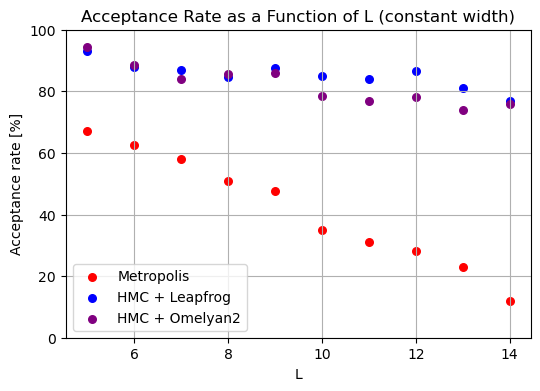
\includegraphics[width=\linewidth]{images/acc_rate_constant_width.png}
        \caption{The dependence of the acceptance rate on the lattice size $L$. The following widths were used: Metropolis w = 0.14 / HMC + Leapfrog w = 0.2 / HMC + Omelyan2 w = 0.44}
        \label{fig:const_width}
    \end{subfigure}
    \hfill 
    \begin{subfigure}[b]{0.48\linewidth}
        \centering
        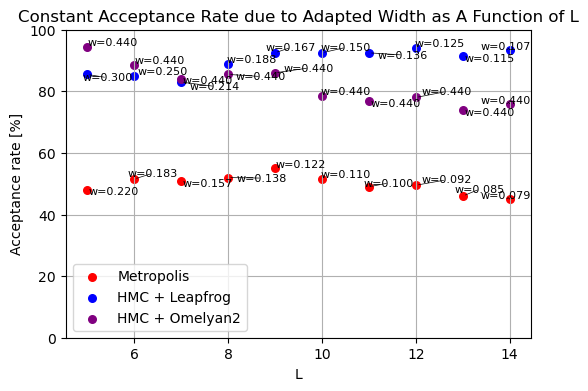
\includegraphics[width=\linewidth]{images/acc_rate_adapted.png}
        \caption{The widths were adapated as a function of $L$ to achieve an acceptance rate of 50\% for Metropolis and 90\% for HMC. The following width functions were used: Metropolis w = 1.1/L / HMC + Leapfrog w = 1.5/L / HMC + Omelyan2 w = 0.44 (const). }
        \label{fig:adapted_width}
    \end{subfigure}
    \caption{Tuning the Acceptance Rates for Different Algorithms}
    \label{fig:tuning_the_acceptance_rates}
\end{figure}
The same tuning parameters were also applied in the Rust implementation. This served as a consistency check to ensure that the Rust version produces results comparable to the Python version.
\section{Monte Carlo Chain Visualization}\label{sec:chain_visual}
In Figure \ref{fig:MC chain}, the Monte Carlo chain of the simulation with different algorithms is shown. The observable displayed is the mean field. These plots are not very useful.
\begin{figure}[H]
    \centering
    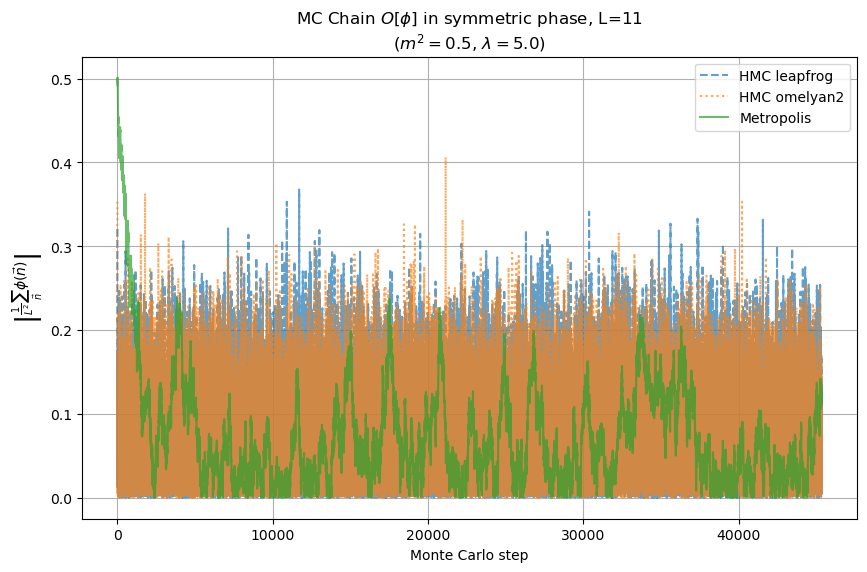
\includegraphics[width=\linewidth]{images/chain.png}
    \caption{Monte Carlo Chain of the Mean Field, Simulation using Different Algorithms}
    \label{fig:MC chain}
\end{figure}
The Metropolis algorithm has the longest thermalization phase, as indicated by the initial drift of the mean field before reaching equilibrium. In contrast, the HMC simulations thermalize more rapidly, likely due to the global updates.
\section{Computational Performance of the Algorithms}\label{sec: data_runtime}
In this section, the computational performance of the different simulation algorithms is compared. The runtimes are shown as a function of lattice size. In addition, the impact of the programming language is investigated comparing Python and Rust versions of the same algorithm. Since lattice simulations are limited by the computational cost, choosing the right algorithm and programming language is crucial. \\\\
The Metropolis and HMC algorithms differ also in their structure and in where most of the computational cost is concentrated. While Metropolis updates are local and inexpensive per step, they suffer from long autocorrelation times. HMC, on the other hand, performs global updates using molecular dynamics trajectories, which are computationally more expensive per iteration but typically yield much faster decorrelation. The statistical independence between configurations is investigated in Section \ref{sec: errs}. \\\\
Furthermore, Python and Rust differ fundamentally in other aspects. Python offers ease of implementation and flexibility but incurs significant overhead due to interpretation and dynamic typing. In contrast, Rust compiles to optimized native code and allows exact control over memory and numerical operations, making it well suited for computationally intensive simulations. In this final project, the computationally intensive algorithms were implemented in Rust and then imported to Python using PyO3 (see \cite{pyo3}). This allows to still use the wonderful Python libraries such as numpy and matplotlib for the analysis and plotting. \\\\
Figures \ref{fig:Pythonruntimes} show the runtimes for the different algorithms in the broken and in the symmetric phase of $\phi^4$-theory using the algorithms implemented in Python. 
\begin{figure}[H]
    \centering
    \begin{subfigure}[b]{0.48\linewidth}
        \centering
        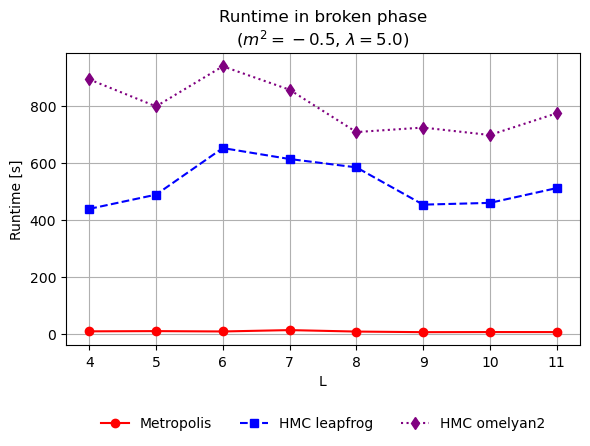
\includegraphics[width=\linewidth]{images/runtimes_Python_broken.png}
        \caption{Broken phase with negative mass}
        \label{fig:broken_python_rt}
    \end{subfigure}
    \hfill 
    \begin{subfigure}[b]{0.48\linewidth}
        \centering
        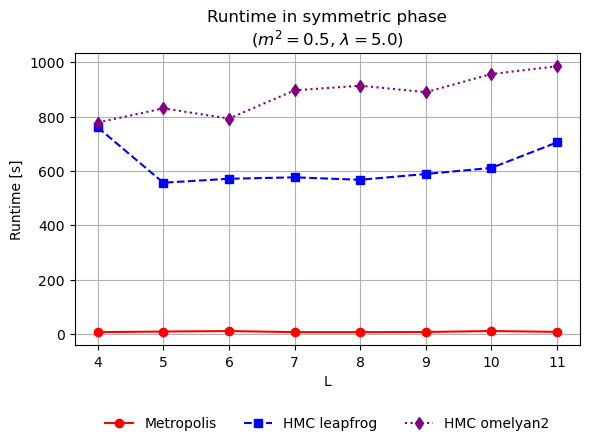
\includegraphics[width=\linewidth]{images/runtimes_Python_symmetric.png}
        \caption{Symmetric phase with positive mass}
        \label{fig:symmetric_python_rt}
    \end{subfigure}
    \caption{Python runtimes}
    \label{fig:Pythonruntimes}
\end{figure}
Figures \ref{fig:Rustruntimes} show the runtimes for the different algorithms in the broken and in the symmetric phase of $\phi^4$-theory using the algorithms implemented in Rust. 
\begin{figure}[H]
    \centering
    \begin{subfigure}[b]{0.48\linewidth}
        \centering
        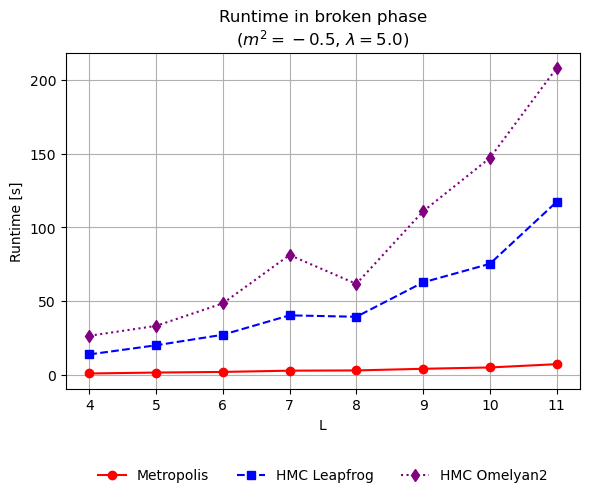
\includegraphics[width=\linewidth]{images/runtimes_Rust_broken.png}
        \caption{Broken phase with negative mass}
        \label{fig:broken_rust_rt}
    \end{subfigure}
    \hfill 
    \begin{subfigure}[b]{0.48\linewidth}
        \centering
        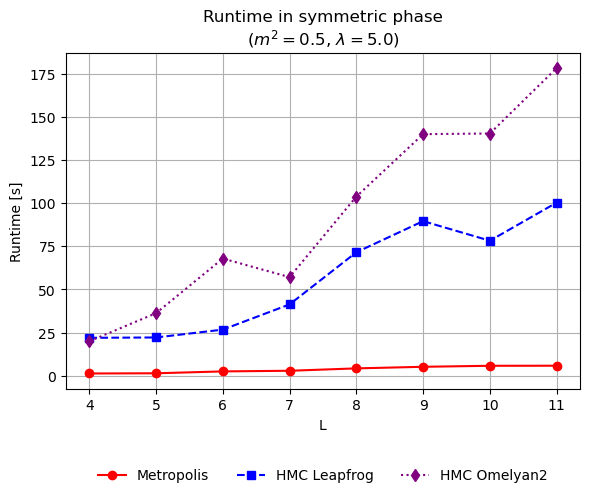
\includegraphics[width=\linewidth]{images/runtimes_Rust_symmetric.png}
        \caption{Symmetric phase with positive mass}
        \label{fig:symmetric_rust_rt}
    \end{subfigure}
    \caption{Rust runtimes}
    \label{fig:Rustruntimes}
\end{figure}
\subsubsection*{Comments on the Results}
\begin{itemize}
    \item Very clearly visible is the speedup achieved by translating the Python code into Rust, the Rust runtimes are a factor of $4-6x$ faster. This was achieved by translating to a more suitable programming language, no efficiency improvements in the algorithms were implemented.
    \item The Metropolis algorithm is the fastest overall, in both Python and Rust. In the Python implementation, the runtime of Metropolis is nearly constant, while in Rust, we observe a slight increase with increasing lattice size $L$. 
    \item The HMC algorithm is significantly slower than the Metropolis algorithm, where the leapfrog integrator is faster than the omelyan2 integrator used in HMC. 
    \item In the Python version, the runtime of HMC for both integrators are more or less constant with the lattice size $L$ for unclear reasons. For the Rust versions of the HMC algorithms, we observe a linear increase of runtime with $L$. This can be explained by the fact that HMC has a larger configuration to update and the equations of motion are more expensive to solve. 
    \item In addition, it can be observed that the runtime in the symmetric phase is higher than in the broken phase of the $\phi^4$-theory. This can be understood in terms of critical slowing down and the structure of field configurations in the two regimes. In the symmetric phase, the system is close to the critical point where the correlation length becomes large. Field updates become more strongly correlated over large distances, the state space is explored more slowly. In contrast, in the broken phase the field fluctuates around one of the two degenerate minima of the potential. The presence of a non-zero vacuum expectation value effectively introduces a mass scale that suppresses long-range correlations. This leads to faster decorrelation of configurations and improved sampling efficiency, reducing the computational cost per independent configuration. \cite{GattingerLang}
\end{itemize}
\section{Measuring Errors and Autocorrelations}\label{sec: errs}
\subsection{Errors}
Accurate error estimations are essential to quantify the reliability of computed observables and to compare benefits of different algorithms. This subsection describes how the statistical errors in Metropolis and HMC using both the leapfrog and omelyan2 integrator evaluated as a function of lattice size $L$. \\\\
The following Figure \ref{fig:python_errors} shows the statistical errors of both phases resulting from the Python implemented algorithms.
\begin{figure}[H]
    \centering
    \begin{subfigure}[b]{0.48\linewidth}
        \centering
        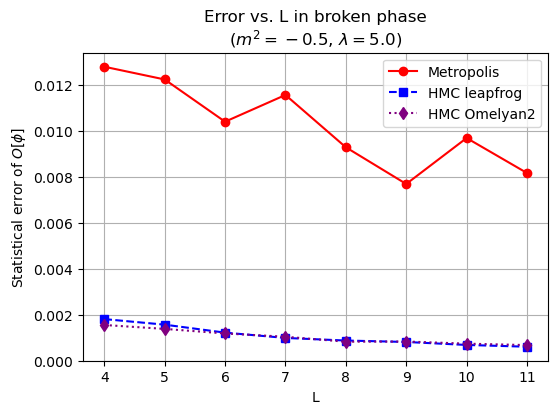
\includegraphics[width=\linewidth]{images/error_Python_broken.png}
        \caption{Broken phase with negative mass}
        \label{fig:broken_python_errors}
    \end{subfigure}
    \hfill 
    \begin{subfigure}[b]{0.48\linewidth}
        \centering
        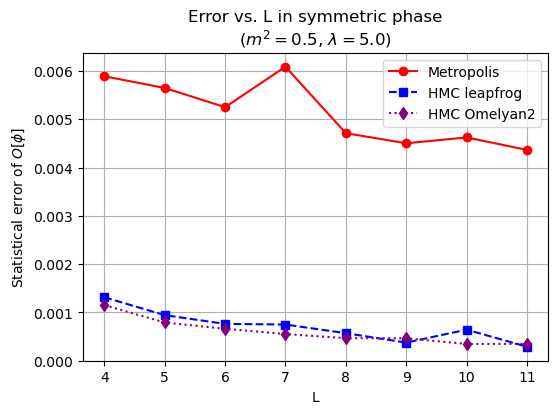
\includegraphics[width=\linewidth]{images/error_Python_symmetric.png}
        \caption{Symmetric phase with positive mass}
        \label{fig:symmetric_python_errors}
    \end{subfigure}
    \caption{Statistical errors as a function of lattice size $L$ for the broken and symmetric phase, algorithms in Python.}
    \label{fig:python_errors}
\end{figure}
The following Figure \ref{fig:rust_errors} shows the statistical errors of both phases resulting from the Rust implemented algorithms.
\begin{figure}[H]
    \centering
    \begin{subfigure}[b]{0.48\linewidth}
        \centering
        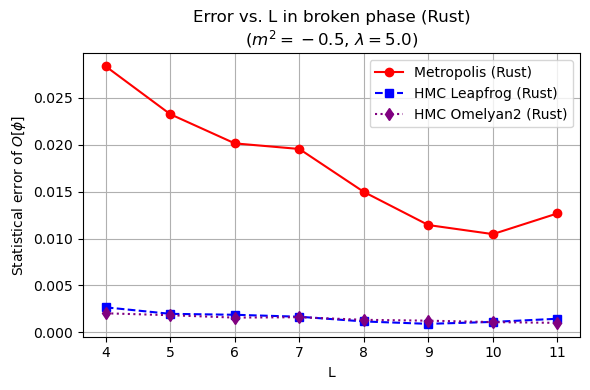
\includegraphics[width=\linewidth]{images/error_Rust_broken.png}
        \caption{Broken phase with negative mass}
        \label{fig:broken_rust_errors}
    \end{subfigure}
    \hfill 
    \begin{subfigure}[b]{0.48\linewidth}
        \centering
        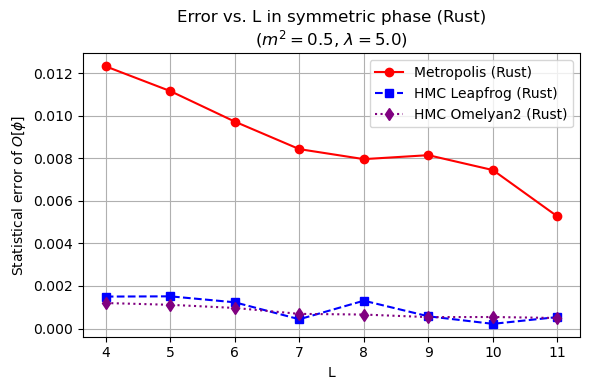
\includegraphics[width=\linewidth]{images/error_Rust_symmetric.png}
        \caption{Symmetric phase with positive mass}
        \label{fig:symmetric_rust_errors}
    \end{subfigure}
    \caption{Statistical Errors as a function of lattice size $L$ for the broken and symmetric phase, algorithms in Rust.}
    \label{fig:rust_errors}
\end{figure}
\subsubsection*{Comments on the Results}
\begin{itemize}
    \item In both the symmetric and broken phases with both Python and Rust, the Metropolis produces significantly larger statistical errors than the HMC algorithm. The HMC algorithm has similar statistical errors for the two different integrators leapfrog and omelyan2. 
    \item For both versions of HMC, the Python and Rust implementations have similar statistical errors. The statistical error of the Metropolis algorithm is approximately twice as large as in the Rust version, for unknown reasons.
    \item In the broken phase the statistical error is significantly larger than in the symmetric phase. This is a consequence of the presence of two degenerate vacua, between which the Monte Carlo simulation can tunnel. These tunneling events lead to long autocorrelation times and large fluctuations of observables, thereby increasing the statistical uncertainty. In contrast, the symmetric phase contains a single stable vacuum and exhibits faster decorrelation.
    \item In all simulations, the statistical error decreases with increasing lattice size $L$. Most likely, this behaviour can be attributed to how the average is computed. The measured observables are spatial averages over the lattice, their variance decreases as $1/V = 1/L^2$. Although autocorrelation times increase with lattice size, especially in the broken phase, the reduction of statistical fluctuations due to averaging over more degrees of freedom dominates in the parameter range considered.
\end{itemize}
\subsection{Autocorrelations}
Autocorrelations measure the memory of a Markov chain and quantify the dependence of successive configurations. High autocorrelation reduces the effective number of independent samples, increasing statistical errors. We discuss the computation of integrated autocorrelation times and their impact on the precision of measured observables.\\\\
The following Figure \ref{fig:autocorr_python} shows the integrated autocorrelation time as a function of lattice size $L$ for the different algorithms implemented in Python. 
\begin{figure}[H]
    \centering
    \begin{subfigure}[b]{0.48\linewidth}
        \centering
        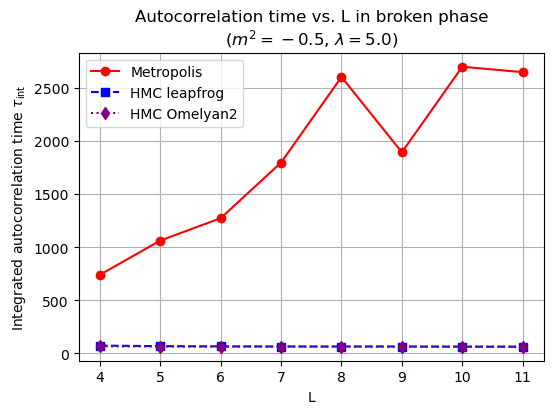
\includegraphics[width=\linewidth]{images/autocorr_Python_broken.png}
        \caption{Broken phase with negative mass}
        \label{fig:broken_python_autocorr}
    \end{subfigure}
    \hfill 
    \begin{subfigure}[b]{0.48\linewidth}
        \centering
        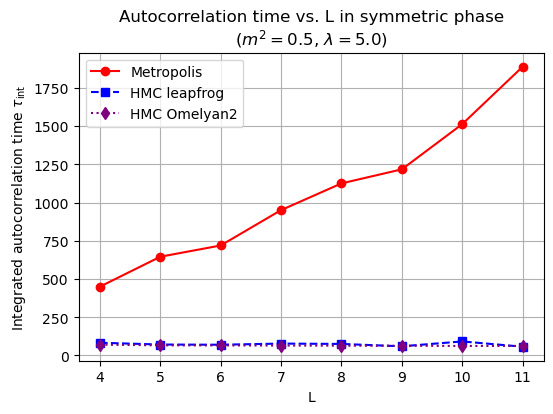
\includegraphics[width=\linewidth]{images/autocorr_Python_symmetric.png}
        \caption{Symmetric phase with positive mass}
        \label{fig:symmetric_python_autocorr}
    \end{subfigure}
    \caption{Autocorrelations as a function of lattice size $L$ for the broken and symmetric phase, algorithms in Python.}
    \label{fig:autocorr_python}
\end{figure}
The following Figure \ref{fig:autocorr_rust} shows the integrated autocorrelation time as a function of lattice size $L$ for the different algorithms implemented in Rust. 
\begin{figure}[H]
    \centering
    \begin{subfigure}[b]{0.48\linewidth}
        \centering
        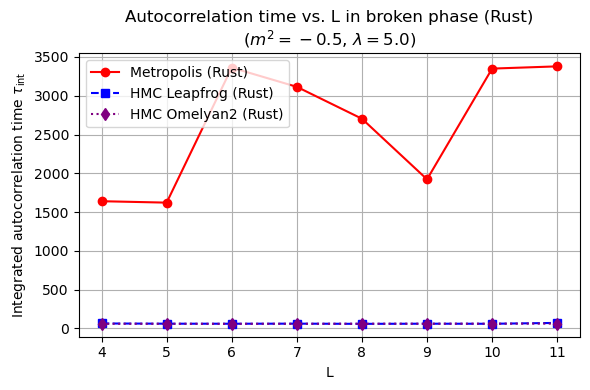
\includegraphics[width=\linewidth]{images/autocorr_Rust_broken.png}
        \caption{Broken phase with negative mass}
        \label{fig:broken_rust_autocorr}
    \end{subfigure}
    \hfill 
    \begin{subfigure}[b]{0.48\linewidth}
        \centering
        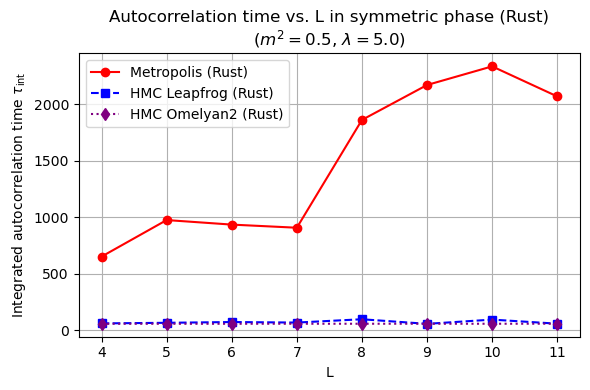
\includegraphics[width=\linewidth]{images/autocorr_Rust_symmetric.png}
        \caption{Symmetric phase with positive mass}
        \label{fig:symmetric_rust_autocorr}
    \end{subfigure}
    \caption{Autocorrelations as a function of lattice size $L$ for the broken and symmetric phase, algorithms in Rust.}
    \label{fig:autocorr_rust}
\end{figure}
\subsubsection*{Comments on the Results}
\begin{itemize}
    \item In all panels, for both Rust and Python, the integrated autocorrelation time increases with lattice size $L$, as expected. This is a manifestation of critical slowing down. As the correlation length grows with the system size, local update algorithms require more steps to decorrelate configurations. The effect is visible for Metropolis, for HMC it is strongly suppressed (since the updates are not local).
    \item The Metropolis algorithm has very large autocorrelation times, which tend to grow with the lattice size $L$. The autocorrelation times for the broken phase are larger, which is expected. In the broken phase, the system has two degenerate minima, local Metropolis updates struggle to tunnel between them. Metropolis becomes impractical for large systems, especially in the broken phase. 
    \item Both HMC variants show dramatically reduced autocorrelation times, nearly flat at $L$. Omelyan2 is systematically slightly lower, since its integration error is smaller. This shows that HMC avoids critical slowing down effectively. Global molecular-dynamics updates decorrelate the system much faster than local update proposals. 
    \item The comparison of the broken and symmetric phase reveals that the broken phase (negative mass square) has larger autocorrelation times overall. The physical reason for that is that the potential has two minima and the configurations must tunnel between two vacua. Metropolis has local updates and therefore almost never tunnels, which leads to large autocorrelation times. HMC tunnels quite efficiently, but still shows a slightly increased autocorrelation. 
    \item When comparing the results from the Rust and Python implementations, the HMC results match mostly. However, there are some discrepancies for the Metropolis algorithm of unknown cause. The physics are expected to be independent of the implementation. Differences could be due to floating-point accumulation order, random number generator differences or a mistake in one of the implementations. The cause could not be identified so far, this needs further investigations.  
\end{itemize}
\section{Comparison of Integrators}\label{sec: int_comparison}
This section contains the result of the analysis comparing the leapfrog and the omelyan2 integrators, which have been described in Chapter \ref{sec: integrators}. 
\subsection{HMC Energy Violations for Symmetric and Broken Phases}
The HMC simulation (Python version only) was run for two phases: the symmetric phase ($m^2 = 0.5$) and the broken phase $(m^2 = -0.5)$, using both the leapfrog and omelyan2 integrators. For each phase, 2000 HMC trajectories on a lattice of size $L = 8$ were computed, using $\varepsilon = 0.1$. \\\\
For each trajectory, we recorded the change in the Hamiltonian between the initial and final configurations. This measures energy conservation of the integrator and is directly related to the HMC acceptance probability.\\\\
The following Table \ref{tab: deltaH_statistics} shows the means and standard deviations of $\Delta H$ for each integrator and for each phase. 
\begin{table}[H]
\centering
\begin{tabular}{lcc}
\hline
\textbf{Phase and Integrator} & \textbf{Mean($\Delta H$)} & \textbf{Std($\Delta H$)} \\
\hline
\textbf{Symmetric Phase} & & \\
\quad Leapfrog & $-3.753\times 10^{-3}$ & $7.684\times 10^{-2}$ \\
\quad Omelyan2 & $-2.297\times 10^{-5}$ & $1.559\times 10^{-3}$ \\
\hline
\textbf{Broken Phase} & & \\
\quad Leapfrog & $-3.252\times 10^{-3}$ & $6.990\times 10^{-2}$ \\
\quad Omelyan2 & $8.146\times 10^{-6}$ & $2.743\times 10^{-3}$ \\
\hline
\end{tabular}
\caption{Statistics of Hamiltonian differences $\Delta H$ for symmetric and broken phases using Leapfrog and Omelyan2 integrators.}
\label{tab: deltaH_statistics}
\end{table}
The following Figures \ref{fig:symmetric_hists} and \ref{fig:broken_hists} show the energy violation distributions for both integrators in the symmetric and broken phase. The scatter plots display $\Delta H$ for each trajectory. 
\begin{figure}[H]
    \centering
    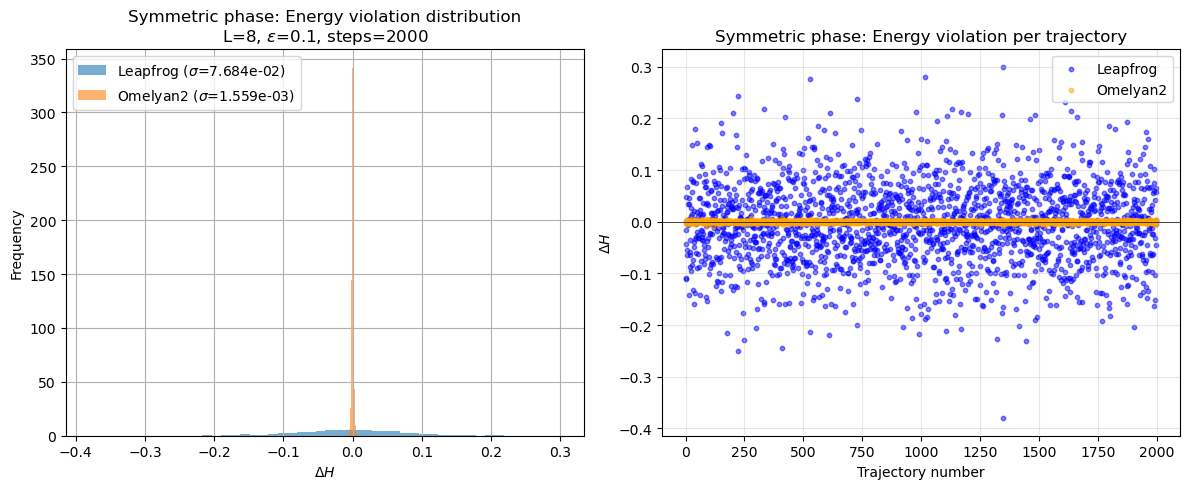
\includegraphics[width=\linewidth]{images/symmetric_hists.png}
    \caption{Distribution of $\Delta H = H_{\text{old}} - H_{\text{new}}$ in the symmetric phase.}
    \label{fig:symmetric_hists}
\end{figure}
\begin{figure}[H]
    \centering
    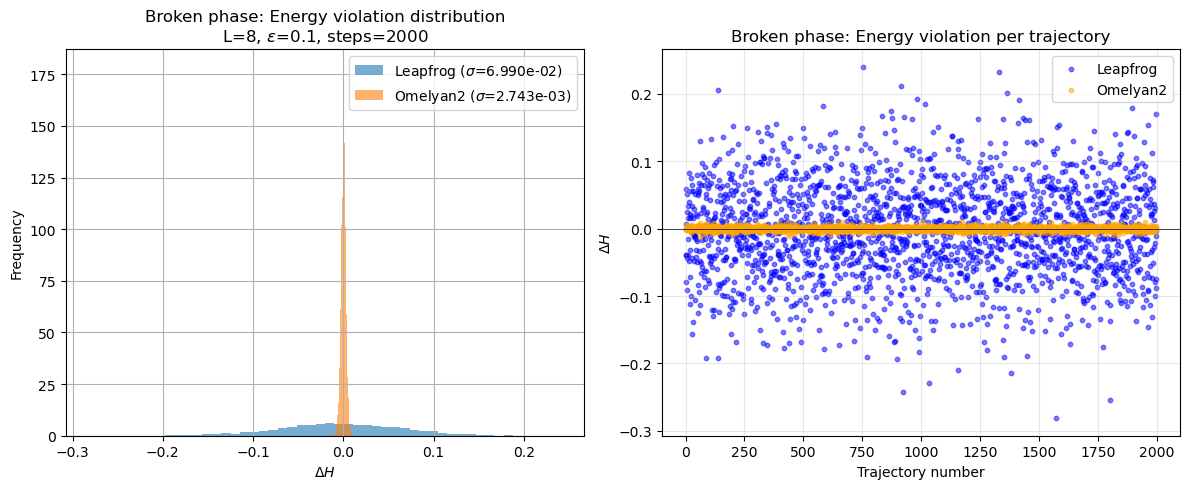
\includegraphics[width=\linewidth]{images/broken_hist.png}
    \caption{Distribution of $\Delta H = H_{\text{old}} - H_{\text{new}}$ in the broken phase.}
    \label{fig:broken_hists}
\end{figure}
\subsubsection*{Comments on the Results}
\begin{itemize}
    \item It is clearly visible in both phases that omelyan2 produces smaller $\Delta H$ fluctuations than leapfrog, indicating better energy conservation.
    \item Leapfrog shows wider distributions and occasional large violations, which could lead to reduced accpetance rate in HMC algorithm.
    \item The difference between symmetric and broken phases is minor, but the analysis confirms the robustness of omelyan2 across different physical regimes.
\end{itemize}
\subsection{Influence of Step Size \texorpdfstring{$\varepsilon$}{eps}}
The HMC simulations were repeated with different step sizes $\varepsilon$. The following Figure \ref{fig:stepsize_comparison} shows the standard deviation of $\Delta H$ as a function of stepsize $\varepsilon$ in both phases and for both leapfrog and omelyan2. 
\begin{figure}[H]
    \centering
    \begin{subfigure}[b]{0.48\linewidth}
        \centering
        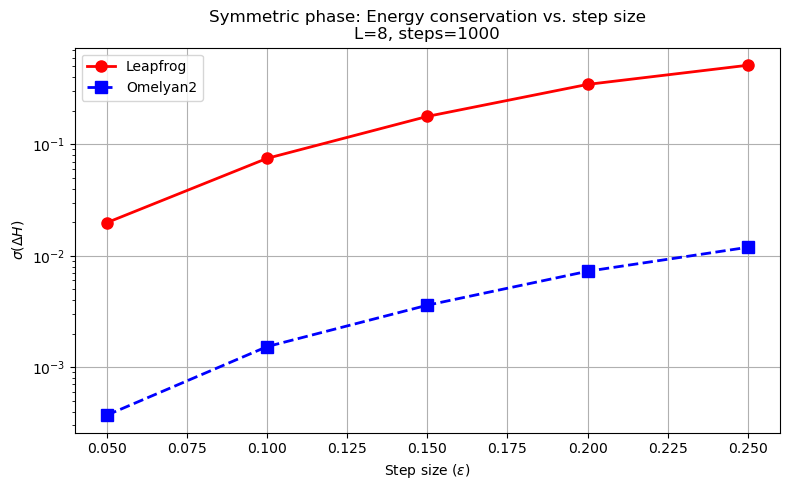
\includegraphics[width=\linewidth]{images/symmetric_stepsize.png}
        \caption{Symmetric phase.}
        \label{fig:symmetric_stepsize}
    \end{subfigure}
    \hfill 
    \begin{subfigure}[b]{0.48\linewidth}
        \centering
        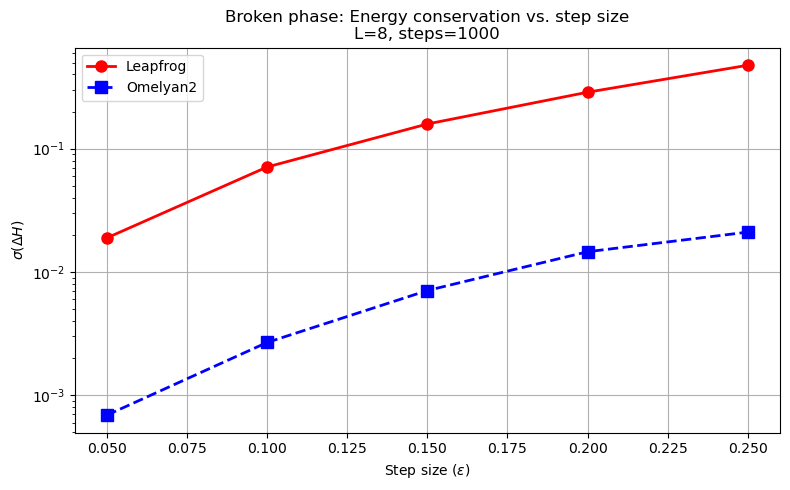
\includegraphics[width=\linewidth]{images/broken_stepsize.png}
        \caption{Broken phase.}
        \label{fig:broken_stepsize}
    \end{subfigure}
    \caption{Standard deviation of $\Delta H$ as a function of stepsize $\varepsilon$. Note that the scale is logarithmic.}
    \label{fig:stepsize_comparison}
\end{figure}
\subsubsection*{Comments on the Results}
\begin{itemize}
    \item There is the expected dependence of $\sigma(\Delta H)$ on the stepsize $\varepsilon$, the standard deviation grows with growing stepsize. 
    \item Both integrators show similar scaling with $\varepsilon$, although omelyan2 maintains consistently lower $\sigma(\Delta H)$ than leapfrog.
    \item The difference between the two phases is minor, indicating that the integrator performance is independent of the physical regime for our parameter choices.
\end{itemize}
\section{Results with the Topological Charge}\label{sec: top_charge_results}
This section is based on \cite{De_2005}. The Metropolis algorithm (Rust version) was used, since it has been extendend to include the option of aperiodic boundary conditions. \\
To study the behaviour of the topological charge as a function of the lattice size, simulations were performed using the Metropolis algorithm for both periodic (PBC) and anti-periodic (APBC) boundary conditions. The number of steps has been increased to $83'160$ (highly composite number, see \cite{wikipedia_highly_composite_number}) to obtain better statistic and clearer results.\\\\
Figure \ref{fig:top_charge} shows the measured topological charge $Q_R$ as a function of the lattice size $L$ for both the broken and symmetric phases, obtained using the Metropolis algorithm with periodic (PBC) and anti-periodic (APBC) boundary conditions. The quantity $Q_R$ measures the difference in topology induced by changing the boundary conditions, and therefore serves as a probe of non-trivial field configurations such as kinks and anti-kinks, see Section \ref{sec:topology}.
\begin{figure}[H]
    \centering
    \begin{subfigure}[b]{0.48\linewidth}
        \centering
        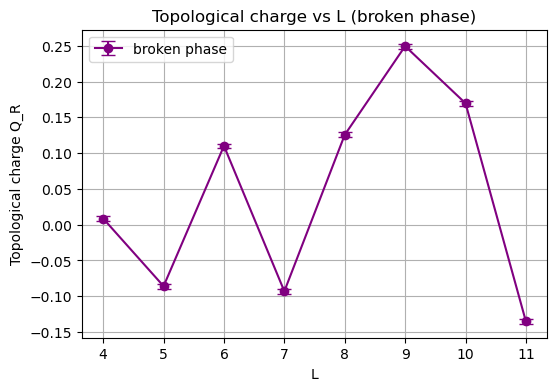
\includegraphics[width=\linewidth]{images/top_charge_broken.png}
        \caption{Topological charge $Q_R$ in the broken phase}
        \label{fig:top_charge_broken}
    \end{subfigure}
    \hfill 
    \begin{subfigure}[b]{0.48\linewidth}
        \centering
        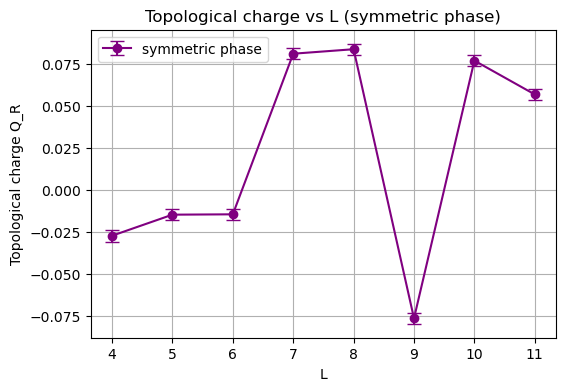
\includegraphics[width=\linewidth]{images/top_charge_symmetric.png}
        \caption{Topological charge $Q_R$ in the symmetric phase}
        \label{fig:top_charge_symmetric}
    \end{subfigure}
    \caption{Topological charge $Q_R$ as a function of lattice size $L$ for the broken and symmetric phases, using PBC and APBC.}
    \label{fig:top_charge}
\end{figure}
\subsubsection*{Comments on the Results}
\begin{itemize}
    \item In the broken phase, the scalar potential possesses two degenerate minima, allowing for topological non-trivial field configurations. This is reflected in the results, $Q_R$ fluctuates around non-zero values, which indicates topological excitations. The sign changes reflect tunneling between the vacua. The magnitude of $Q_R$ is clearly larger than in the symmetric phase. We observe no dependence on the lattice size $L$. 
    \item In the symmetric phase, the potential has one minimum and topological effects are suppressed. This is cleary visible, the fluctuations have a much smaller magnitude and are close to zero. The fluctuations can likely be explained by statistical noise. 
    \item Overall, the behaviour of $Q_R$ in both phases agrees with the expectations of $\phi^4$ theory. Nontrivial topological structures appear only when degenerate minima exist (broken phase), and vanish in the symmetric phase.
\end{itemize}
\chapter{Conclusions}
In this final project, the Metropolis and HMC algorithms were implemented for the two-dimensional $\phi^4$-theory and the performance was compared across different integrators, programming languages and physical regimes. 
\\\\
Before performing the main anaylsis, the algorithms were tuned to the correct acceptance rates, see Section \ref{sec: tuning}. The Metropolis algorithm was tuned to approximately 50\% acceptance rate, HMC was tuned to around 90\%. 
\\\\
In Section \ref{sec:chain_visual}, the Monte Carlo history of the mean field observable was visualized to assess thermalization. These plots were found not be of great quantitative usefulness. However, it could be concluded that the Metropolis algorithm has the longest thermalization time, since it has local updates, in contrast to the global molecular-dynamics HMC updates. 
\\\\
Section \ref{sec: data_runtime} focused on the run times of the algorithms (Metropolis vs. HMC with both integrators) implemented in two programming languages (Python vs. Python). Translating the code from Python to Rust yielded a substantial speedup of a factor $4-6$. It was conlcluded that implementing expensive tasks in Rust is beneficial. The use of PyO3 enables a convenient framework in which performance-critical components are written in Rust, while data analysis and visualization remain in Python. In general, the Metropolis algorithm is computationally inexpensive. Solving the equations of motions for HMC numerically is much more expensive, the use of integrator does not influence the run time of HMC dramatically. Additionally, it was observed that the run time depends on the phase of the system, which can be interpreted in terms of critical slowing down. 
\\\\
In Section \ref{sec: errs}, statistical errors and integrated autocorrelation times were analyzed. The results show that the Metropolis algorithm produces significantly larger statistical errors than HMC. Both leapfrog and omelyan2 integrators exhibit similar statistical uncertainties, but HMC clearly outperforms Metropolis in terms of autocorrelation times. The statistical errors are larger in the broken phase than in the symmetric phase, which can be attributed to the presence of two degenerate vacua. Furthermore, while statistical errors decrease with increasing lattice size $L$, the integrated autocorrelation time increases, reflecting critical slowing down. This effect is particularly pronounced for Metropolis, whereas HMC suppresses it efficiently. Discrepancies between Python and Rust implementations are not fully explained, this needs further investigations, since errors and autocorrelation times should be independent of the programming language. 
\\\\
Section \ref{sec: int_comparison} examines the performance of the integrators leapfrog and omelyan2 in HMC. The HMC algorithm, with both leapfrog and omelyan2 integrators, demonstrates excellent energy conservation and high acceptance rates, particularly with the omelyan2 integrator. Our results show that omelyan2 consistently produces smaller Hamiltonian violations than leapfrog, confirming its improved stability and robustness across the symmetric and broken phases. The step size $\varepsilon$ strongly influences energy conservation, with the standard deviation of $\Delta H$ growing as approximately $\varepsilon^2$.
\\\\
The study of the topological charge $Q_R$ using the Rust Metropolis implementation further illustrates the physical differences between the phases. In the broken phase, non-trivial topological excitations such as kinks and anti-kinks emerge, with $Q_R$ fluctuating around non-zero values and occasionally changing sign due to tunneling events. In the symmetric phase, these topological effects are suppressed, and $Q_R$ remains close to zero, as expected.
\\\\
Overall, our analysis confirms that the choice of algorithm, integrator, and programming language has a strong impact on simulation efficiency, statistical precision, and energy conservation. HMC with omelyan2 integrator in Rust provides the most favorable combination of accuracy, efficiency, and low autocorrelation.
\section{Possible Extensions}
Here are a few suggestions on how to extend this final project: 
\begin{itemize}
    \item The current code base of this project is written such that the action of the theory could be exchanged with relatively simply, allowing the code to be used for different, more realistic theories than scalar $\phi^4$ theory. However, it would require some effort to implement fermions or gauge fields. 
    \item While the leapfrog and especially omelyan2 integrators for HMC are robust and stable, higher order integrators could be added in order to further reduce integration errors and to improve energy conservation. 
    \item It would be interesting to study more sophisticated observables. Beyond the mean field and the topological charge, one could measure for example correclation functions or susceptibilities. 
    \item The Rust implementation could be improved significantly using parallelization or GPU acceleration, allowing simulations on larger lattices or large parameter scans. Combining high-performance Rust code with Python plotting and analysis by means of PyO3 provides many possibilities for LFT. 
\end{itemize}
\printbibliography

\end{document}